\documentclass{book}
\usepackage[a4paper,top=2.5cm,bottom=2.5cm,left=2.5cm,right=2.5cm]{geometry}
\usepackage{makeidx}
\usepackage{natbib}
\usepackage{graphicx}
\usepackage{multicol}
\usepackage{float}
\usepackage{listings}
\usepackage{color}
\usepackage{ifthen}
\usepackage[table]{xcolor}
\usepackage{textcomp}
\usepackage{alltt}
\usepackage{ifpdf}
\ifpdf
\usepackage[pdftex,
            pagebackref=true,
            colorlinks=true,
            linkcolor=blue,
            unicode
           ]{hyperref}
\else
\usepackage[ps2pdf,
            pagebackref=true,
            colorlinks=true,
            linkcolor=blue,
            unicode
           ]{hyperref}
\usepackage{pspicture}
\fi
\usepackage[utf8]{inputenc}
\usepackage{mathptmx}
\usepackage[scaled=.90]{helvet}
\usepackage{courier}
\usepackage{sectsty}
\usepackage{amssymb}
\usepackage[titles]{tocloft}
\usepackage{doxygen}
\lstset{language=C++,inputencoding=utf8,basicstyle=\footnotesize,breaklines=true,breakatwhitespace=true,tabsize=4,numbers=left }
\makeindex
\setcounter{tocdepth}{3}
\renewcommand{\footrulewidth}{0.4pt}
\renewcommand{\familydefault}{\sfdefault}
\hfuzz=15pt
\setlength{\emergencystretch}{15pt}
\hbadness=750
\tolerance=750
\begin{document}
\hypersetup{pageanchor=false,citecolor=blue}
\begin{titlepage}
\vspace*{7cm}
\begin{center}
{\Large Virtual Piggy Unity Plugin }\\
\vspace*{1cm}
{\large Generated by Doxygen 1.8.2}\\
\vspace*{0.5cm}
{\small Mon Oct 15 2012 10:47:59}\\
\end{center}
\end{titlepage}
\clearemptydoublepage
\pagenumbering{roman}
\tableofcontents
\clearemptydoublepage
\pagenumbering{arabic}
\hypersetup{pageanchor=true,citecolor=blue}
\chapter{Main Page}
\label{index}\hypertarget{index}{}\hypertarget{index_intro_sec}{}\section{Introduction}\label{index_intro_sec}
The Virtual Piggy Unity Plugin allows developers to enable kids to manage and spend money within a parent-\/controlled environment that also allows merchants to sell to them while complying with the Children's Online Privacy Protection Act (C\-O\-P\-P\-A).\hypertarget{index_install_sec}{}\section{Installation}\label{index_install_sec}
\hypertarget{index_step1}{}\subsection{Step 1\-:}\label{index_step1}
Download and Import Virtual Piggy Plugin Unity Package \hypertarget{index_step2}{}\subsection{Step 2\-:}\label{index_step2}
Enter Merchant Identifier, A\-P\-I Key and Environment in settings by accessing Virtual Piggy Project Settings Window (Virtual Piggy $>$ Project Settings) \hypertarget{index_step3}{}\subsection{Step 3\-:}\label{index_step3}
Bring in \hyperlink{class_virtual_piggy_event_listener}{Virtual\-Piggy\-Event\-Listener}, \hyperlink{class_virtual_piggy_manager}{Virtual\-Piggy\-Manager} and \hyperlink{class_virtual_piggy_g_u_i}{Virtual\-Piggy\-G\-U\-I} prefabs into Scene \hypertarget{index_step4}{}\subsection{Step 4\-:}\label{index_step4}
Build for Web and upload it to your server. \hypertarget{index_usage_sec}{}\section{Usage}\label{index_usage_sec}
For an example on Usage please see the Example Scene located in Plugins $>$ \hyperlink{class_virtual_piggy}{Virtual\-Piggy} $>$ Example and the Test\-Store.\-cs class

If you'd like to clear the current User Token in the Editor, simple select the Virtual Piggy $>$ Clear Token drop down.

Included is a default G\-U\-I\-S\-Kin for the G\-U\-I. It is localed in Plugins $>$ \hyperlink{class_virtual_piggy}{Virtual\-Piggy} $>$ Skin For more information on Modifying the G\-U\-I please see \hyperlink{modifying_the_gui}{Modifying the G\-U\-I} 
\chapter{Modifying the G\-U\-I}
\label{modifying_the_gui}
\hypertarget{modifying_the_gui}{}
If you have experience with Unity G\-U\-I\-Skins then you probably already know how to modify the default G\-U\-I. Simply make a new G\-U\-I\-Skin and apply it to the Virtual Piggy Skin value on \hyperlink{class_virtual_piggy_g_u_i}{Virtual\-Piggy\-G\-U\-I}. If you're not experienced with Unity's G\-U\-I\-Skins, continue reading.

If you'd like to change the look of the G\-U\-I included with the Plugin, you have a couple of choices. Included is a G\-U\-I\-Skin already put together for you. This is located in Plugins $>$ \hyperlink{class_virtual_piggy}{Virtual\-Piggy} $>$ Skin You may also create your own G\-U\-I\-Skin.

If you want to use your own G\-U\-I\-Skin, all you need to do is create a new G\-U\-I\-Skin and apply it to \hyperlink{class_virtual_piggy_g_u_i}{Virtual\-Piggy\-G\-U\-I}. You'll want to edit the Button, Label and Text\-Field elements.

The \hyperlink{class_virtual_piggy_g_u_i}{Virtual\-Piggy\-G\-U\-I} object also uses 16 custom styles. The easiest way to maintain the references to these is to Duplicate one of the existing G\-U\-I\-Skins. Then all you need to do is swap in the textures/fonts you want to use. The styles that this skin uses are\-: Login Button, Transaction\-Message, Success\-Indicator, fail\-Indicator, progress\-Indicator, fader, Transaction\-Ask\-Message, close\-Login, Yes\-Button, No\-Button, logo\-Backer, bg-\/border, bg, required\-Text, Login\-Text and grey\-Line.

If you want to scale the size of the gui \hyperlink{class_virtual_piggy_g_u_i}{Virtual\-Piggy\-G\-U\-I} has a \char`\"{}gui\-Scale\char`\"{} member that you can use adjust. 
\chapter{Hierarchical Index}
\section{Class Hierarchy}
This inheritance list is sorted roughly, but not completely, alphabetically\-:\begin{DoxyCompactList}
\item \contentsline{section}{Virtual\-Piggy.\-Login\-Response}{\pageref{class_virtual_piggy_1_1_login_response}}{}
\item Mono\-Behaviour\begin{DoxyCompactList}
\item \contentsline{section}{Virtual\-Piggy\-Event\-Listener}{\pageref{class_virtual_piggy_event_listener}}{}
\item \contentsline{section}{Virtual\-Piggy\-G\-U\-I}{\pageref{class_virtual_piggy_g_u_i}}{}
\item \contentsline{section}{Virtual\-Piggy\-Manager}{\pageref{class_virtual_piggy_manager}}{}
\end{DoxyCompactList}
\item \contentsline{section}{Virtual\-Piggy.\-S\-O\-A\-P\-Request}{\pageref{class_virtual_piggy_1_1_s_o_a_p_request}}{}
\item \contentsline{section}{Virtual\-Piggy.\-Transaction\-Response}{\pageref{class_virtual_piggy_1_1_transaction_response}}{}
\item \contentsline{section}{Virtual\-Piggy}{\pageref{class_virtual_piggy}}{}
\item \contentsline{section}{Virtual\-Piggy\-Settings}{\pageref{class_virtual_piggy_settings}}{}
\end{DoxyCompactList}

\chapter{Class Index}
\section{Class List}
Here are the classes, structs, unions and interfaces with brief descriptions\-:\begin{DoxyCompactList}
\item\contentsline{section}{\hyperlink{class_virtual_piggy_1_1_login_response}{Virtual\-Piggy.\-Login\-Response} \\*Login response object }{\pageref{class_virtual_piggy_1_1_login_response}}{}
\item\contentsline{section}{\hyperlink{class_virtual_piggy_1_1_s_o_a_p_request}{Virtual\-Piggy.\-S\-O\-A\-P\-Request} \\*Stores S\-O\-A\-P Request data. }{\pageref{class_virtual_piggy_1_1_s_o_a_p_request}}{}
\item\contentsline{section}{\hyperlink{class_virtual_piggy_1_1_transaction_response}{Virtual\-Piggy.\-Transaction\-Response} \\*Transaction response object }{\pageref{class_virtual_piggy_1_1_transaction_response}}{}
\item\contentsline{section}{\hyperlink{class_virtual_piggy}{Virtual\-Piggy} \\*Virtual Piggy A\-P\-I }{\pageref{class_virtual_piggy}}{}
\item\contentsline{section}{\hyperlink{class_virtual_piggy_event_listener}{Virtual\-Piggy\-Event\-Listener} }{\pageref{class_virtual_piggy_event_listener}}{}
\item\contentsline{section}{\hyperlink{class_virtual_piggy_g_u_i}{Virtual\-Piggy\-G\-U\-I} \\*This class is responsible for rendering the Virtual Piggy Login/\-Transaction Dialog }{\pageref{class_virtual_piggy_g_u_i}}{}
\item\contentsline{section}{\hyperlink{class_virtual_piggy_manager}{Virtual\-Piggy\-Manager} }{\pageref{class_virtual_piggy_manager}}{}
\item\contentsline{section}{\hyperlink{class_virtual_piggy_settings}{Virtual\-Piggy\-Settings} \\*Virtual Piggy Plugin Settings. These are set using the Project Settings window, accessed from Menu Virtual Piggy$>$Project Settings }{\pageref{class_virtual_piggy_settings}}{}
\end{DoxyCompactList}

\chapter{Class Documentation}
\hypertarget{class_virtual_piggy_1_1_login_response}{\section{Virtual\-Piggy.\-Login\-Response Class Reference}
\label{class_virtual_piggy_1_1_login_response}\index{Virtual\-Piggy.\-Login\-Response@{Virtual\-Piggy.\-Login\-Response}}
}


Login response object  


\subsection*{Public Attributes}
\begin{DoxyCompactItemize}
\item 
\hypertarget{class_virtual_piggy_1_1_login_response_a889c215d8f5d8a8586f49d9adf486997}{string {\bfseries Token}}\label{class_virtual_piggy_1_1_login_response_a889c215d8f5d8a8586f49d9adf486997}

\item 
\hypertarget{class_virtual_piggy_1_1_login_response_ae8a1614599cdbc1b0cfd98e7c40f780b}{string {\bfseries Error\-Message}}\label{class_virtual_piggy_1_1_login_response_ae8a1614599cdbc1b0cfd98e7c40f780b}

\item 
\hypertarget{class_virtual_piggy_1_1_login_response_acbae2fa63321be3f8f111eac5c4205d8}{string {\bfseries User\-Type}}\label{class_virtual_piggy_1_1_login_response_acbae2fa63321be3f8f111eac5c4205d8}

\end{DoxyCompactItemize}


\subsection{Detailed Description}
Login response object 



The documentation for this class was generated from the following file\-:\begin{DoxyCompactItemize}
\item 
/\-Users/\-C\-P\-X-\/\-Hackintosh01/\-Virtual Piggy Plugin/\-Assets/\-Plugins/\-Virtual\-Piggy/Virtual\-Piggy.\-cs\end{DoxyCompactItemize}

\hypertarget{class_virtual_piggy_1_1_s_o_a_p_request}{\section{Virtual\-Piggy.\-S\-O\-A\-P\-Request Class Reference}
\label{class_virtual_piggy_1_1_s_o_a_p_request}\index{Virtual\-Piggy.\-S\-O\-A\-P\-Request@{Virtual\-Piggy.\-S\-O\-A\-P\-Request}}
}


Stores S\-O\-A\-P Request data.  


\subsection*{Public Attributes}
\begin{DoxyCompactItemize}
\item 
\hypertarget{class_virtual_piggy_1_1_s_o_a_p_request_aadb6951b6e40c08a758b2fc69bb16771}{string {\bfseries request}}\label{class_virtual_piggy_1_1_s_o_a_p_request_aadb6951b6e40c08a758b2fc69bb16771}

\item 
\hypertarget{class_virtual_piggy_1_1_s_o_a_p_request_a6241a2e66694a8a9509cd96e65c8b369}{\hyperlink{class_virtual_piggy_adca55d9dcf3fd7482dacac0ec3258afd}{R\-E\-Q\-U\-E\-S\-T\-\_\-\-T\-Y\-P\-E} {\bfseries request\-Type}}\label{class_virtual_piggy_1_1_s_o_a_p_request_a6241a2e66694a8a9509cd96e65c8b369}

\item 
\hypertarget{class_virtual_piggy_1_1_s_o_a_p_request_aa05beab351aef8cc9ca04f09a8c6ce51}{Hashtable {\bfseries headers}}\label{class_virtual_piggy_1_1_s_o_a_p_request_aa05beab351aef8cc9ca04f09a8c6ce51}

\end{DoxyCompactItemize}


\subsection{Detailed Description}
Stores S\-O\-A\-P Request data. 



The documentation for this class was generated from the following file\-:\begin{DoxyCompactItemize}
\item 
/\-Users/\-C\-P\-X-\/\-Hackintosh01/\-Virtual Piggy Plugin/\-Assets/\-Plugins/\-Virtual\-Piggy/Virtual\-Piggy.\-cs\end{DoxyCompactItemize}

\hypertarget{class_virtual_piggy_1_1_transaction_response}{\section{Virtual\-Piggy.\-Transaction\-Response Class Reference}
\label{class_virtual_piggy_1_1_transaction_response}\index{Virtual\-Piggy.\-Transaction\-Response@{Virtual\-Piggy.\-Transaction\-Response}}
}


Transaction response object  


\subsection*{Public Attributes}
\begin{DoxyCompactItemize}
\item 
\hypertarget{class_virtual_piggy_1_1_transaction_response_ab7b2a07aae6d9d39ca288d6712e9af13}{string {\bfseries Data\-Xml}}\label{class_virtual_piggy_1_1_transaction_response_ab7b2a07aae6d9d39ca288d6712e9af13}

\item 
\hypertarget{class_virtual_piggy_1_1_transaction_response_a68a49209ae2dbb9854c8ad8bfac6e130}{string {\bfseries Error\-Message}}\label{class_virtual_piggy_1_1_transaction_response_a68a49209ae2dbb9854c8ad8bfac6e130}

\item 
\hypertarget{class_virtual_piggy_1_1_transaction_response_a62ef9079bb88991e313b6b9fe60b7251}{string {\bfseries Transaction\-Identifier}}\label{class_virtual_piggy_1_1_transaction_response_a62ef9079bb88991e313b6b9fe60b7251}

\item 
\hypertarget{class_virtual_piggy_1_1_transaction_response_ab1a48c5351474f984a6dbe6aca79adb0}{string {\bfseries Transaction\-Status}}\label{class_virtual_piggy_1_1_transaction_response_ab1a48c5351474f984a6dbe6aca79adb0}

\item 
\hypertarget{class_virtual_piggy_1_1_transaction_response_a82e3175e280b55c49dbb92ab45f0af04}{bool {\bfseries Status}}\label{class_virtual_piggy_1_1_transaction_response_a82e3175e280b55c49dbb92ab45f0af04}

\end{DoxyCompactItemize}


\subsection{Detailed Description}
Transaction response object 



The documentation for this class was generated from the following file\-:\begin{DoxyCompactItemize}
\item 
/\-Users/\-C\-P\-X-\/\-Hackintosh01/\-Virtual Piggy Plugin/\-Assets/\-Plugins/\-Virtual\-Piggy/Virtual\-Piggy.\-cs\end{DoxyCompactItemize}

\hypertarget{class_virtual_piggy}{\section{Virtual\-Piggy Class Reference}
\label{class_virtual_piggy}\index{Virtual\-Piggy@{Virtual\-Piggy}}
}


Virtual Piggy A\-P\-I  


\subsection*{Classes}
\begin{DoxyCompactItemize}
\item 
class \hyperlink{class_virtual_piggy_1_1_login_response}{Login\-Response}
\begin{DoxyCompactList}\small\item\em Login response object \end{DoxyCompactList}\item 
class \hyperlink{class_virtual_piggy_1_1_s_o_a_p_request}{S\-O\-A\-P\-Request}
\begin{DoxyCompactList}\small\item\em Stores S\-O\-A\-P Request data. \end{DoxyCompactList}\item 
class \hyperlink{class_virtual_piggy_1_1_transaction_response}{Transaction\-Response}
\begin{DoxyCompactList}\small\item\em Transaction response object \end{DoxyCompactList}\end{DoxyCompactItemize}
\subsection*{Public Types}
\begin{DoxyCompactItemize}
\item 
enum \hyperlink{class_virtual_piggy_adca55d9dcf3fd7482dacac0ec3258afd}{R\-E\-Q\-U\-E\-S\-T\-\_\-\-T\-Y\-P\-E} \{ {\bfseries A\-U\-T\-H\-E\-N\-T\-I\-C\-A\-T\-E\-\_\-\-U\-S\-E\-R}, 
{\bfseries A\-U\-T\-H\-E\-N\-T\-I\-C\-A\-T\-E\-\_\-\-C\-H\-I\-L\-D}, 
{\bfseries T\-R\-A\-N\-S\-A\-C\-T\-I\-O\-N}
 \}
\begin{DoxyCompactList}\small\item\em Type of Request being made to Virtual Piggy backend \end{DoxyCompactList}\end{DoxyCompactItemize}
\subsection*{Static Public Member Functions}
\begin{DoxyCompactItemize}
\item 
static void \hyperlink{class_virtual_piggy_a9d88b45c735cc1d66f5b1b040d6f06f2}{Initialize} ()
\begin{DoxyCompactList}\small\item\em Initialize Virtual Piggy A\-P\-I \end{DoxyCompactList}\item 
static void \hyperlink{class_virtual_piggy_ac6801551dbc6b114cf51c40b9f38703d}{Logout} ()
\begin{DoxyCompactList}\small\item\em Log user out of Virtual Piggy \end{DoxyCompactList}\item 
\hypertarget{class_virtual_piggy_a6848953790e21496550c6d6d0a34c4e4}{static void {\bfseries Login} (Action$<$ \hyperlink{class_virtual_piggy_1_1_login_response}{Login\-Response} $>$ success, Action$<$ string $>$ fail)}\label{class_virtual_piggy_a6848953790e21496550c6d6d0a34c4e4}

\item 
static void \hyperlink{class_virtual_piggy_a5af0f57e5b47349aa2130ff7930d2d17}{Authenticate\-User} (string user\-Name, string password)
\begin{DoxyCompactList}\small\item\em Authenticates the user. \end{DoxyCompactList}\item 
static void \hyperlink{class_virtual_piggy_a3db7e0e95d00378043520e4c83b17fd8}{Authenticate\-Child} (string user\-Name, string password)
\begin{DoxyCompactList}\small\item\em Authenticates the child. \end{DoxyCompactList}\item 
static void \hyperlink{class_virtual_piggy_ab40b96be4aaf8a8f20d97293b1bdda7d}{Process\-Transaction} (string product\-Name, float price, int quantity, string product\-Description, bool prompt\-For\-Purchase=false)
\begin{DoxyCompactList}\small\item\em Processes a transaction. \end{DoxyCompactList}\end{DoxyCompactItemize}
\subsection*{Properties}
\begin{DoxyCompactItemize}
\item 
static string \hyperlink{class_virtual_piggy_a1dbe43b28ff22f55ee3be3b6eb54def1}{Merchant\-I\-D}\hspace{0.3cm}{\ttfamily  \mbox{[}get, set\mbox{]}}
\begin{DoxyCompactList}\small\item\em Merchant Identifier accessor \end{DoxyCompactList}\item 
static string \hyperlink{class_virtual_piggy_a01aab4ab653d5d9ca572d28ff5d63aa8}{A\-P\-I\-Key}\hspace{0.3cm}{\ttfamily  \mbox{[}get, set\mbox{]}}
\begin{DoxyCompactList}\small\item\em A\-P\-I Key accessor \end{DoxyCompactList}\item 
static string \hyperlink{class_virtual_piggy_a27549028a152d40ddf293705da935a9b}{Token}\hspace{0.3cm}{\ttfamily  \mbox{[}get, set\mbox{]}}
\begin{DoxyCompactList}\small\item\em Current logged in user's token \end{DoxyCompactList}\item 
static bool \hyperlink{class_virtual_piggy_af0ab9dea29cfb35855cd75d80a652900}{Is\-Logged\-In}\hspace{0.3cm}{\ttfamily  \mbox{[}get\mbox{]}}
\begin{DoxyCompactList}\small\item\em Gets a value indicating whether this instance is logged in. \end{DoxyCompactList}\end{DoxyCompactItemize}


\subsection{Detailed Description}
Virtual Piggy A\-P\-I 



\subsection{Member Enumeration Documentation}
\hypertarget{class_virtual_piggy_adca55d9dcf3fd7482dacac0ec3258afd}{\index{Virtual\-Piggy@{Virtual\-Piggy}!R\-E\-Q\-U\-E\-S\-T\-\_\-\-T\-Y\-P\-E@{R\-E\-Q\-U\-E\-S\-T\-\_\-\-T\-Y\-P\-E}}
\index{R\-E\-Q\-U\-E\-S\-T\-\_\-\-T\-Y\-P\-E@{R\-E\-Q\-U\-E\-S\-T\-\_\-\-T\-Y\-P\-E}!VirtualPiggy@{Virtual\-Piggy}}
\subsubsection[{R\-E\-Q\-U\-E\-S\-T\-\_\-\-T\-Y\-P\-E}]{\setlength{\rightskip}{0pt plus 5cm}enum {\bf Virtual\-Piggy.\-R\-E\-Q\-U\-E\-S\-T\-\_\-\-T\-Y\-P\-E}}}\label{class_virtual_piggy_adca55d9dcf3fd7482dacac0ec3258afd}


Type of Request being made to Virtual Piggy backend 



\subsection{Member Function Documentation}
\hypertarget{class_virtual_piggy_a3db7e0e95d00378043520e4c83b17fd8}{\index{Virtual\-Piggy@{Virtual\-Piggy}!Authenticate\-Child@{Authenticate\-Child}}
\index{Authenticate\-Child@{Authenticate\-Child}!VirtualPiggy@{Virtual\-Piggy}}
\subsubsection[{Authenticate\-Child}]{\setlength{\rightskip}{0pt plus 5cm}static void Virtual\-Piggy.\-Authenticate\-Child (
\begin{DoxyParamCaption}
\item[{string}]{user\-Name, }
\item[{string}]{password}
\end{DoxyParamCaption}
)\hspace{0.3cm}{\ttfamily [static]}}}\label{class_virtual_piggy_a3db7e0e95d00378043520e4c83b17fd8}


Authenticates the child. 


\begin{DoxyParams}{Parameters}
{\em user\-Name} & User name. \\
\hline
{\em password} & Password. \\
\hline
\end{DoxyParams}
\hypertarget{class_virtual_piggy_a5af0f57e5b47349aa2130ff7930d2d17}{\index{Virtual\-Piggy@{Virtual\-Piggy}!Authenticate\-User@{Authenticate\-User}}
\index{Authenticate\-User@{Authenticate\-User}!VirtualPiggy@{Virtual\-Piggy}}
\subsubsection[{Authenticate\-User}]{\setlength{\rightskip}{0pt plus 5cm}static void Virtual\-Piggy.\-Authenticate\-User (
\begin{DoxyParamCaption}
\item[{string}]{user\-Name, }
\item[{string}]{password}
\end{DoxyParamCaption}
)\hspace{0.3cm}{\ttfamily [static]}}}\label{class_virtual_piggy_a5af0f57e5b47349aa2130ff7930d2d17}


Authenticates the user. 


\begin{DoxyParams}{Parameters}
{\em user\-Name} & User name. \\
\hline
{\em password} & Password. \\
\hline
\end{DoxyParams}
\hypertarget{class_virtual_piggy_a9d88b45c735cc1d66f5b1b040d6f06f2}{\index{Virtual\-Piggy@{Virtual\-Piggy}!Initialize@{Initialize}}
\index{Initialize@{Initialize}!VirtualPiggy@{Virtual\-Piggy}}
\subsubsection[{Initialize}]{\setlength{\rightskip}{0pt plus 5cm}static void Virtual\-Piggy.\-Initialize (
\begin{DoxyParamCaption}
{}
\end{DoxyParamCaption}
)\hspace{0.3cm}{\ttfamily [static]}}}\label{class_virtual_piggy_a9d88b45c735cc1d66f5b1b040d6f06f2}


Initialize Virtual Piggy A\-P\-I 

\hypertarget{class_virtual_piggy_ac6801551dbc6b114cf51c40b9f38703d}{\index{Virtual\-Piggy@{Virtual\-Piggy}!Logout@{Logout}}
\index{Logout@{Logout}!VirtualPiggy@{Virtual\-Piggy}}
\subsubsection[{Logout}]{\setlength{\rightskip}{0pt plus 5cm}static void Virtual\-Piggy.\-Logout (
\begin{DoxyParamCaption}
{}
\end{DoxyParamCaption}
)\hspace{0.3cm}{\ttfamily [static]}}}\label{class_virtual_piggy_ac6801551dbc6b114cf51c40b9f38703d}


Log user out of Virtual Piggy 

\hypertarget{class_virtual_piggy_ab40b96be4aaf8a8f20d97293b1bdda7d}{\index{Virtual\-Piggy@{Virtual\-Piggy}!Process\-Transaction@{Process\-Transaction}}
\index{Process\-Transaction@{Process\-Transaction}!VirtualPiggy@{Virtual\-Piggy}}
\subsubsection[{Process\-Transaction}]{\setlength{\rightskip}{0pt plus 5cm}static void Virtual\-Piggy.\-Process\-Transaction (
\begin{DoxyParamCaption}
\item[{string}]{product\-Name, }
\item[{float}]{price, }
\item[{int}]{quantity, }
\item[{string}]{product\-Description, }
\item[{bool}]{prompt\-For\-Purchase = {\ttfamily false}}
\end{DoxyParamCaption}
)\hspace{0.3cm}{\ttfamily [static]}}}\label{class_virtual_piggy_ab40b96be4aaf8a8f20d97293b1bdda7d}


Processes a transaction. 


\begin{DoxyParams}{Parameters}
{\em product\-Name} & Product name. \\
\hline
{\em price} & Price. \\
\hline
{\em quantity} & Quantity. \\
\hline
{\em product\-Description} & Product description. \\
\hline
{\em prompt\-For\-Purchase} & Prompt user for purchase. \\
\hline
\end{DoxyParams}


\subsection{Property Documentation}
\hypertarget{class_virtual_piggy_a01aab4ab653d5d9ca572d28ff5d63aa8}{\index{Virtual\-Piggy@{Virtual\-Piggy}!A\-P\-I\-Key@{A\-P\-I\-Key}}
\index{A\-P\-I\-Key@{A\-P\-I\-Key}!VirtualPiggy@{Virtual\-Piggy}}
\subsubsection[{A\-P\-I\-Key}]{\setlength{\rightskip}{0pt plus 5cm}string Virtual\-Piggy.\-A\-P\-I\-Key\hspace{0.3cm}{\ttfamily [static]}, {\ttfamily [get]}, {\ttfamily [set]}}}\label{class_virtual_piggy_a01aab4ab653d5d9ca572d28ff5d63aa8}


A\-P\-I Key accessor 

\hypertarget{class_virtual_piggy_af0ab9dea29cfb35855cd75d80a652900}{\index{Virtual\-Piggy@{Virtual\-Piggy}!Is\-Logged\-In@{Is\-Logged\-In}}
\index{Is\-Logged\-In@{Is\-Logged\-In}!VirtualPiggy@{Virtual\-Piggy}}
\subsubsection[{Is\-Logged\-In}]{\setlength{\rightskip}{0pt plus 5cm}bool Virtual\-Piggy.\-Is\-Logged\-In\hspace{0.3cm}{\ttfamily [static]}, {\ttfamily [get]}}}\label{class_virtual_piggy_af0ab9dea29cfb35855cd75d80a652900}


Gets a value indicating whether this instance is logged in. 

{\ttfamily true} if this instance is logged in; otherwise, {\ttfamily false}. \hypertarget{class_virtual_piggy_a1dbe43b28ff22f55ee3be3b6eb54def1}{\index{Virtual\-Piggy@{Virtual\-Piggy}!Merchant\-I\-D@{Merchant\-I\-D}}
\index{Merchant\-I\-D@{Merchant\-I\-D}!VirtualPiggy@{Virtual\-Piggy}}
\subsubsection[{Merchant\-I\-D}]{\setlength{\rightskip}{0pt plus 5cm}string Virtual\-Piggy.\-Merchant\-I\-D\hspace{0.3cm}{\ttfamily [static]}, {\ttfamily [get]}, {\ttfamily [set]}}}\label{class_virtual_piggy_a1dbe43b28ff22f55ee3be3b6eb54def1}


Merchant Identifier accessor 

\hypertarget{class_virtual_piggy_a27549028a152d40ddf293705da935a9b}{\index{Virtual\-Piggy@{Virtual\-Piggy}!Token@{Token}}
\index{Token@{Token}!VirtualPiggy@{Virtual\-Piggy}}
\subsubsection[{Token}]{\setlength{\rightskip}{0pt plus 5cm}string Virtual\-Piggy.\-Token\hspace{0.3cm}{\ttfamily [static]}, {\ttfamily [get]}, {\ttfamily [set]}}}\label{class_virtual_piggy_a27549028a152d40ddf293705da935a9b}


Current logged in user's token 



The documentation for this class was generated from the following file\-:\begin{DoxyCompactItemize}
\item 
/\-Users/\-C\-P\-X-\/\-Hackintosh01/\-Virtual Piggy Plugin/\-Assets/\-Plugins/\-Virtual\-Piggy/Virtual\-Piggy.\-cs\end{DoxyCompactItemize}

\hypertarget{class_virtual_piggy_event_listener}{\section{Virtual\-Piggy\-Event\-Listener Class Reference}
\label{class_virtual_piggy_event_listener}\index{Virtual\-Piggy\-Event\-Listener@{Virtual\-Piggy\-Event\-Listener}}
}
Inheritance diagram for Virtual\-Piggy\-Event\-Listener\-:\begin{figure}[H]
\begin{center}
\leavevmode
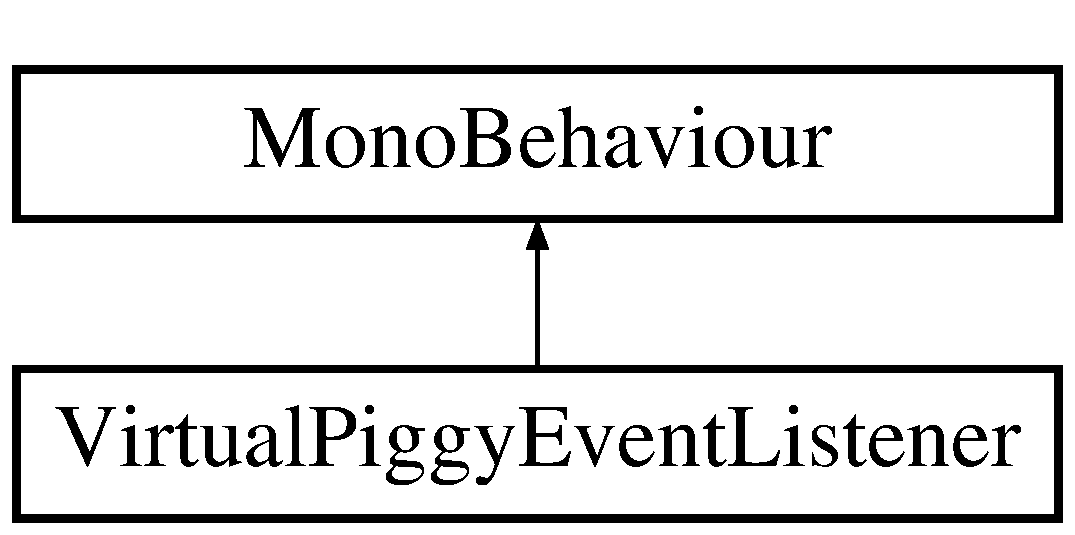
\includegraphics[height=2.000000cm]{class_virtual_piggy_event_listener}
\end{center}
\end{figure}
\subsection*{Events}
\begin{DoxyCompactItemize}
\item 
static Action\\*
$<$ \hyperlink{class_virtual_piggy_1_1_login_response}{Virtual\-Piggy.\-Login\-Response} $>$ \hyperlink{class_virtual_piggy_event_listener_a37e2f432ebe9efec24f8d21c8e9433c7}{on\-Login\-Success}
\begin{DoxyCompactList}\small\item\em Occurs when logged in successfully. \end{DoxyCompactList}\item 
static Action$<$ string $>$ \hyperlink{class_virtual_piggy_event_listener_a580e126cb0048aaa4daafa0de836f4bb}{on\-Login\-Fail}
\begin{DoxyCompactList}\small\item\em Occurs when login fails. \end{DoxyCompactList}\item 
static Action \hyperlink{class_virtual_piggy_event_listener_ad0e8ac1d1b94df9f5dc1e3e7ec755ecc}{on\-Login\-Dismissed}
\begin{DoxyCompactList}\small\item\em Occurs when login is dismissed. \end{DoxyCompactList}\item 
static Action\\*
$<$ \hyperlink{class_virtual_piggy_1_1_transaction_response}{Virtual\-Piggy.\-Transaction\-Response} $>$ \hyperlink{class_virtual_piggy_event_listener_a58bcbdf1f33687818fd58a40bd07eeb3}{on\-Transaction\-Success}
\begin{DoxyCompactList}\small\item\em Occurs on transaction success. \end{DoxyCompactList}\item 
static Action$<$ string $>$ \hyperlink{class_virtual_piggy_event_listener_a2bb1383f9e7fff212815aa3c838180cf}{on\-Transaction\-Fail}
\begin{DoxyCompactList}\small\item\em Occurs on transaction fail. \end{DoxyCompactList}\end{DoxyCompactItemize}


\subsection{Event Documentation}
\hypertarget{class_virtual_piggy_event_listener_ad0e8ac1d1b94df9f5dc1e3e7ec755ecc}{\index{Virtual\-Piggy\-Event\-Listener@{Virtual\-Piggy\-Event\-Listener}!on\-Login\-Dismissed@{on\-Login\-Dismissed}}
\index{on\-Login\-Dismissed@{on\-Login\-Dismissed}!VirtualPiggyEventListener@{Virtual\-Piggy\-Event\-Listener}}
\subsubsection[{on\-Login\-Dismissed}]{\setlength{\rightskip}{0pt plus 5cm}Action Virtual\-Piggy\-Event\-Listener.\-on\-Login\-Dismissed\hspace{0.3cm}{\ttfamily [static]}}}\label{class_virtual_piggy_event_listener_ad0e8ac1d1b94df9f5dc1e3e7ec755ecc}


Occurs when login is dismissed. 

\hypertarget{class_virtual_piggy_event_listener_a580e126cb0048aaa4daafa0de836f4bb}{\index{Virtual\-Piggy\-Event\-Listener@{Virtual\-Piggy\-Event\-Listener}!on\-Login\-Fail@{on\-Login\-Fail}}
\index{on\-Login\-Fail@{on\-Login\-Fail}!VirtualPiggyEventListener@{Virtual\-Piggy\-Event\-Listener}}
\subsubsection[{on\-Login\-Fail}]{\setlength{\rightskip}{0pt plus 5cm}Action$<$string$>$ Virtual\-Piggy\-Event\-Listener.\-on\-Login\-Fail\hspace{0.3cm}{\ttfamily [static]}}}\label{class_virtual_piggy_event_listener_a580e126cb0048aaa4daafa0de836f4bb}


Occurs when login fails. 

\hypertarget{class_virtual_piggy_event_listener_a37e2f432ebe9efec24f8d21c8e9433c7}{\index{Virtual\-Piggy\-Event\-Listener@{Virtual\-Piggy\-Event\-Listener}!on\-Login\-Success@{on\-Login\-Success}}
\index{on\-Login\-Success@{on\-Login\-Success}!VirtualPiggyEventListener@{Virtual\-Piggy\-Event\-Listener}}
\subsubsection[{on\-Login\-Success}]{\setlength{\rightskip}{0pt plus 5cm}Action$<${\bf Virtual\-Piggy.\-Login\-Response}$>$ Virtual\-Piggy\-Event\-Listener.\-on\-Login\-Success\hspace{0.3cm}{\ttfamily [static]}}}\label{class_virtual_piggy_event_listener_a37e2f432ebe9efec24f8d21c8e9433c7}


Occurs when logged in successfully. 

\hypertarget{class_virtual_piggy_event_listener_a2bb1383f9e7fff212815aa3c838180cf}{\index{Virtual\-Piggy\-Event\-Listener@{Virtual\-Piggy\-Event\-Listener}!on\-Transaction\-Fail@{on\-Transaction\-Fail}}
\index{on\-Transaction\-Fail@{on\-Transaction\-Fail}!VirtualPiggyEventListener@{Virtual\-Piggy\-Event\-Listener}}
\subsubsection[{on\-Transaction\-Fail}]{\setlength{\rightskip}{0pt plus 5cm}Action$<$string$>$ Virtual\-Piggy\-Event\-Listener.\-on\-Transaction\-Fail\hspace{0.3cm}{\ttfamily [static]}}}\label{class_virtual_piggy_event_listener_a2bb1383f9e7fff212815aa3c838180cf}


Occurs on transaction fail. 

\hypertarget{class_virtual_piggy_event_listener_a58bcbdf1f33687818fd58a40bd07eeb3}{\index{Virtual\-Piggy\-Event\-Listener@{Virtual\-Piggy\-Event\-Listener}!on\-Transaction\-Success@{on\-Transaction\-Success}}
\index{on\-Transaction\-Success@{on\-Transaction\-Success}!VirtualPiggyEventListener@{Virtual\-Piggy\-Event\-Listener}}
\subsubsection[{on\-Transaction\-Success}]{\setlength{\rightskip}{0pt plus 5cm}Action$<${\bf Virtual\-Piggy.\-Transaction\-Response}$>$ Virtual\-Piggy\-Event\-Listener.\-on\-Transaction\-Success\hspace{0.3cm}{\ttfamily [static]}}}\label{class_virtual_piggy_event_listener_a58bcbdf1f33687818fd58a40bd07eeb3}


Occurs on transaction success. 



The documentation for this class was generated from the following file\-:\begin{DoxyCompactItemize}
\item 
/\-Users/\-C\-P\-X-\/\-Hackintosh01/\-Virtual Piggy Plugin/\-Assets/\-Plugins/\-Virtual\-Piggy/Virtual\-Piggy\-Event\-Listener.\-cs\end{DoxyCompactItemize}

\hypertarget{class_virtual_piggy_g_u_i}{\section{Virtual\-Piggy\-G\-U\-I Class Reference}
\label{class_virtual_piggy_g_u_i}\index{Virtual\-Piggy\-G\-U\-I@{Virtual\-Piggy\-G\-U\-I}}
}


This class is responsible for rendering the Virtual Piggy Login/\-Transaction Dialog  


Inheritance diagram for Virtual\-Piggy\-G\-U\-I\-:\begin{figure}[H]
\begin{center}
\leavevmode
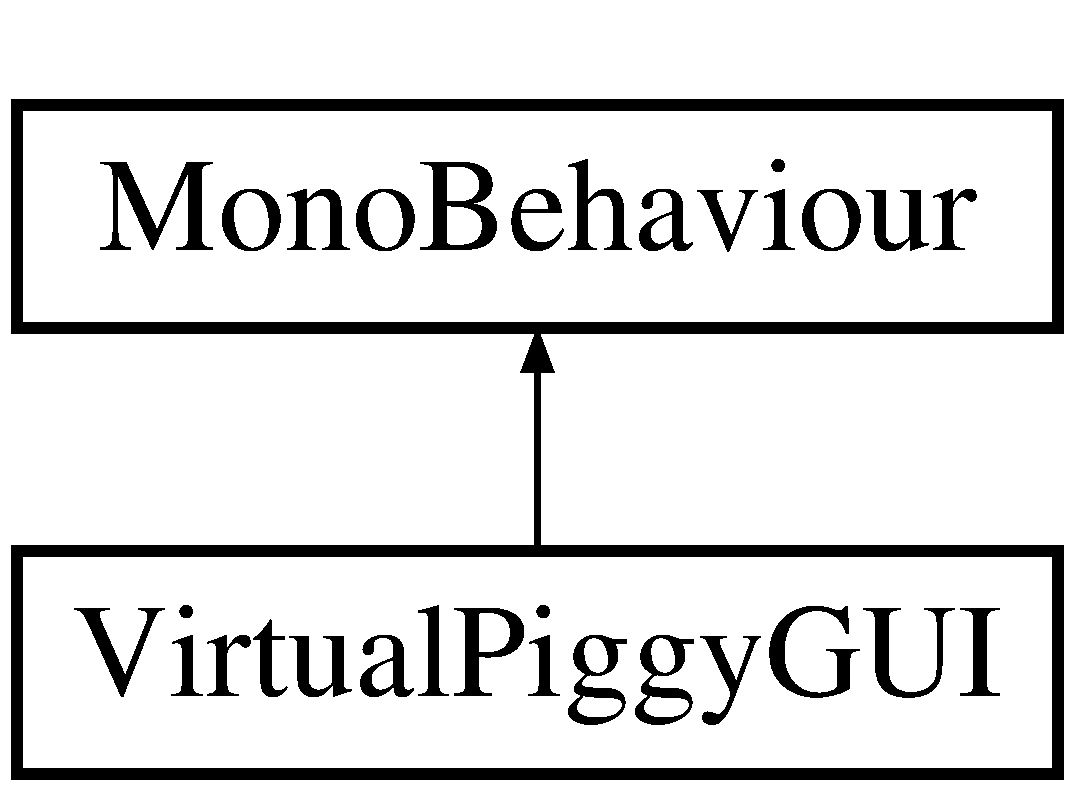
\includegraphics[height=2.000000cm]{class_virtual_piggy_g_u_i}
\end{center}
\end{figure}
\subsection*{Public Types}
\begin{DoxyCompactItemize}
\item 
enum \hyperlink{class_virtual_piggy_g_u_i_acfc203ccd9a2018fb6c1e53ebe244c8d}{S\-T\-A\-T\-E} \{ \\*
{\bfseries L\-O\-G\-I\-N}, 
{\bfseries A\-U\-T\-H\-E\-N\-T\-I\-C\-A\-T\-I\-N\-G}, 
{\bfseries T\-R\-A\-N\-S\-A\-C\-T\-I\-O\-N\-\_\-\-A\-S\-K}, 
{\bfseries T\-R\-A\-N\-S\-A\-C\-T\-I\-O\-N\-\_\-\-I\-N\-\_\-\-P\-R\-O\-G\-R\-E\-S\-S}, 
\\*
{\bfseries T\-R\-A\-N\-S\-A\-C\-T\-I\-O\-N\-\_\-\-C\-O\-M\-P\-L\-E\-T\-E}, 
{\bfseries T\-R\-A\-N\-S\-A\-C\-T\-I\-O\-N\-\_\-\-F\-A\-I\-L}, 
{\bfseries N\-O\-N\-E}
 \}
\begin{DoxyCompactList}\small\item\em States of G\-U\-I \end{DoxyCompactList}\end{DoxyCompactItemize}
\subsection*{Public Member Functions}
\begin{DoxyCompactItemize}
\item 
void \hyperlink{class_virtual_piggy_g_u_i_a0c3dfdd1f04f8c54aae45eb6e9dacbb6}{Prompt\-For\-Purchase} (string product\-Name, float price, int quantity, string product\-Description)
\begin{DoxyCompactList}\small\item\em Prompt the user before performing Transaction \end{DoxyCompactList}\item 
void \hyperlink{class_virtual_piggy_g_u_i_a8120fba4e910a063603d0acccc4d618d}{Show\-Transaction\-Progress} ()
\begin{DoxyCompactList}\small\item\em Shows the transaction progress. \end{DoxyCompactList}\item 
void \hyperlink{class_virtual_piggy_g_u_i_ae0fe2ccfef48ccfbcfa3861418081046}{Login\-Dialog} (Action$<$ \hyperlink{class_virtual_piggy_1_1_login_response}{Virtual\-Piggy.\-Login\-Response} $>$ success\-Callback, Action$<$ string $>$ fail\-Callback)
\begin{DoxyCompactList}\small\item\em Display login dialog to user. \end{DoxyCompactList}\end{DoxyCompactItemize}
\subsection*{Public Attributes}
\begin{DoxyCompactItemize}
\item 
G\-U\-I\-Skin \hyperlink{class_virtual_piggy_g_u_i_a6d7bdaef0dd72024639f51008c202130}{gui\-Skin}
\begin{DoxyCompactList}\small\item\em The G\-U\-I skin that will be used for G\-U\-I \end{DoxyCompactList}\item 
Animation \hyperlink{class_virtual_piggy_g_u_i_a0fcb59d1bf578d056d0bc123a89e75f0}{bounce\-In\-Animation}
\begin{DoxyCompactList}\small\item\em Animation that is used for the login Dialog \end{DoxyCompactList}\item 
float \hyperlink{class_virtual_piggy_g_u_i_acef2dc6ac83a1dd3b72796fcce046934}{gui\-Scale} = 1.\-0f
\begin{DoxyCompactList}\small\item\em Scale of G\-U\-I \end{DoxyCompactList}\item 
float \hyperlink{class_virtual_piggy_g_u_i_adb759917612421d1475ba86a7d6dc056}{animation\-Scale} = 1.\-0f
\begin{DoxyCompactList}\small\item\em scale used in login animation, hidden in inspector \end{DoxyCompactList}\item 
Vector2 \hyperlink{class_virtual_piggy_g_u_i_a7464dcd32b13809bf7893ce3ad858bdf}{loading\-Indicator\-Texture\-Coordinates}
\begin{DoxyCompactList}\small\item\em The loading indicator texture coordinates. \end{DoxyCompactList}\end{DoxyCompactItemize}


\subsection{Detailed Description}
This class is responsible for rendering the Virtual Piggy Login/\-Transaction Dialog 



\subsection{Member Enumeration Documentation}
\hypertarget{class_virtual_piggy_g_u_i_acfc203ccd9a2018fb6c1e53ebe244c8d}{\index{Virtual\-Piggy\-G\-U\-I@{Virtual\-Piggy\-G\-U\-I}!S\-T\-A\-T\-E@{S\-T\-A\-T\-E}}
\index{S\-T\-A\-T\-E@{S\-T\-A\-T\-E}!VirtualPiggyGUI@{Virtual\-Piggy\-G\-U\-I}}
\subsubsection[{S\-T\-A\-T\-E}]{\setlength{\rightskip}{0pt plus 5cm}enum {\bf Virtual\-Piggy\-G\-U\-I.\-S\-T\-A\-T\-E}}}\label{class_virtual_piggy_g_u_i_acfc203ccd9a2018fb6c1e53ebe244c8d}


States of G\-U\-I 



\subsection{Member Function Documentation}
\hypertarget{class_virtual_piggy_g_u_i_ae0fe2ccfef48ccfbcfa3861418081046}{\index{Virtual\-Piggy\-G\-U\-I@{Virtual\-Piggy\-G\-U\-I}!Login\-Dialog@{Login\-Dialog}}
\index{Login\-Dialog@{Login\-Dialog}!VirtualPiggyGUI@{Virtual\-Piggy\-G\-U\-I}}
\subsubsection[{Login\-Dialog}]{\setlength{\rightskip}{0pt plus 5cm}void Virtual\-Piggy\-G\-U\-I.\-Login\-Dialog (
\begin{DoxyParamCaption}
\item[{Action$<$ {\bf Virtual\-Piggy.\-Login\-Response} $>$}]{success\-Callback, }
\item[{Action$<$ string $>$}]{fail\-Callback}
\end{DoxyParamCaption}
)}}\label{class_virtual_piggy_g_u_i_ae0fe2ccfef48ccfbcfa3861418081046}


Display login dialog to user. 


\begin{DoxyParams}{Parameters}
{\em success\-Callback} & Success callback. \\
\hline
{\em fail\-Callback} & Fail callback. \\
\hline
\end{DoxyParams}
\hypertarget{class_virtual_piggy_g_u_i_a0c3dfdd1f04f8c54aae45eb6e9dacbb6}{\index{Virtual\-Piggy\-G\-U\-I@{Virtual\-Piggy\-G\-U\-I}!Prompt\-For\-Purchase@{Prompt\-For\-Purchase}}
\index{Prompt\-For\-Purchase@{Prompt\-For\-Purchase}!VirtualPiggyGUI@{Virtual\-Piggy\-G\-U\-I}}
\subsubsection[{Prompt\-For\-Purchase}]{\setlength{\rightskip}{0pt plus 5cm}void Virtual\-Piggy\-G\-U\-I.\-Prompt\-For\-Purchase (
\begin{DoxyParamCaption}
\item[{string}]{product\-Name, }
\item[{float}]{price, }
\item[{int}]{quantity, }
\item[{string}]{product\-Description}
\end{DoxyParamCaption}
)}}\label{class_virtual_piggy_g_u_i_a0c3dfdd1f04f8c54aae45eb6e9dacbb6}


Prompt the user before performing Transaction 


\begin{DoxyParams}{Parameters}
{\em product\-Name} & Product name. \\
\hline
{\em price} & Price. \\
\hline
{\em quantity} & Quantity. \\
\hline
{\em product\-Description} & Product description. \\
\hline
\end{DoxyParams}
\hypertarget{class_virtual_piggy_g_u_i_a8120fba4e910a063603d0acccc4d618d}{\index{Virtual\-Piggy\-G\-U\-I@{Virtual\-Piggy\-G\-U\-I}!Show\-Transaction\-Progress@{Show\-Transaction\-Progress}}
\index{Show\-Transaction\-Progress@{Show\-Transaction\-Progress}!VirtualPiggyGUI@{Virtual\-Piggy\-G\-U\-I}}
\subsubsection[{Show\-Transaction\-Progress}]{\setlength{\rightskip}{0pt plus 5cm}void Virtual\-Piggy\-G\-U\-I.\-Show\-Transaction\-Progress (
\begin{DoxyParamCaption}
{}
\end{DoxyParamCaption}
)}}\label{class_virtual_piggy_g_u_i_a8120fba4e910a063603d0acccc4d618d}


Shows the transaction progress. 



\subsection{Member Data Documentation}
\hypertarget{class_virtual_piggy_g_u_i_adb759917612421d1475ba86a7d6dc056}{\index{Virtual\-Piggy\-G\-U\-I@{Virtual\-Piggy\-G\-U\-I}!animation\-Scale@{animation\-Scale}}
\index{animation\-Scale@{animation\-Scale}!VirtualPiggyGUI@{Virtual\-Piggy\-G\-U\-I}}
\subsubsection[{animation\-Scale}]{\setlength{\rightskip}{0pt plus 5cm}float Virtual\-Piggy\-G\-U\-I.\-animation\-Scale = 1.\-0f}}\label{class_virtual_piggy_g_u_i_adb759917612421d1475ba86a7d6dc056}


scale used in login animation, hidden in inspector 

\hypertarget{class_virtual_piggy_g_u_i_a0fcb59d1bf578d056d0bc123a89e75f0}{\index{Virtual\-Piggy\-G\-U\-I@{Virtual\-Piggy\-G\-U\-I}!bounce\-In\-Animation@{bounce\-In\-Animation}}
\index{bounce\-In\-Animation@{bounce\-In\-Animation}!VirtualPiggyGUI@{Virtual\-Piggy\-G\-U\-I}}
\subsubsection[{bounce\-In\-Animation}]{\setlength{\rightskip}{0pt plus 5cm}Animation Virtual\-Piggy\-G\-U\-I.\-bounce\-In\-Animation}}\label{class_virtual_piggy_g_u_i_a0fcb59d1bf578d056d0bc123a89e75f0}


Animation that is used for the login Dialog 

\hypertarget{class_virtual_piggy_g_u_i_acef2dc6ac83a1dd3b72796fcce046934}{\index{Virtual\-Piggy\-G\-U\-I@{Virtual\-Piggy\-G\-U\-I}!gui\-Scale@{gui\-Scale}}
\index{gui\-Scale@{gui\-Scale}!VirtualPiggyGUI@{Virtual\-Piggy\-G\-U\-I}}
\subsubsection[{gui\-Scale}]{\setlength{\rightskip}{0pt plus 5cm}float Virtual\-Piggy\-G\-U\-I.\-gui\-Scale = 1.\-0f}}\label{class_virtual_piggy_g_u_i_acef2dc6ac83a1dd3b72796fcce046934}


Scale of G\-U\-I 

\hypertarget{class_virtual_piggy_g_u_i_a6d7bdaef0dd72024639f51008c202130}{\index{Virtual\-Piggy\-G\-U\-I@{Virtual\-Piggy\-G\-U\-I}!gui\-Skin@{gui\-Skin}}
\index{gui\-Skin@{gui\-Skin}!VirtualPiggyGUI@{Virtual\-Piggy\-G\-U\-I}}
\subsubsection[{gui\-Skin}]{\setlength{\rightskip}{0pt plus 5cm}G\-U\-I\-Skin Virtual\-Piggy\-G\-U\-I.\-gui\-Skin}}\label{class_virtual_piggy_g_u_i_a6d7bdaef0dd72024639f51008c202130}


The G\-U\-I skin that will be used for G\-U\-I 

\hypertarget{class_virtual_piggy_g_u_i_a7464dcd32b13809bf7893ce3ad858bdf}{\index{Virtual\-Piggy\-G\-U\-I@{Virtual\-Piggy\-G\-U\-I}!loading\-Indicator\-Texture\-Coordinates@{loading\-Indicator\-Texture\-Coordinates}}
\index{loading\-Indicator\-Texture\-Coordinates@{loading\-Indicator\-Texture\-Coordinates}!VirtualPiggyGUI@{Virtual\-Piggy\-G\-U\-I}}
\subsubsection[{loading\-Indicator\-Texture\-Coordinates}]{\setlength{\rightskip}{0pt plus 5cm}Vector2 Virtual\-Piggy\-G\-U\-I.\-loading\-Indicator\-Texture\-Coordinates}}\label{class_virtual_piggy_g_u_i_a7464dcd32b13809bf7893ce3ad858bdf}


The loading indicator texture coordinates. 



The documentation for this class was generated from the following file\-:\begin{DoxyCompactItemize}
\item 
/\-Users/\-C\-P\-X-\/\-Hackintosh01/\-Virtual Piggy Plugin/\-Assets/\-Plugins/\-Virtual\-Piggy/Virtual\-Piggy\-G\-U\-I.\-cs\end{DoxyCompactItemize}

\hypertarget{class_virtual_piggy_manager}{\section{Virtual\-Piggy\-Manager Class Reference}
\label{class_virtual_piggy_manager}\index{Virtual\-Piggy\-Manager@{Virtual\-Piggy\-Manager}}
}
Inheritance diagram for Virtual\-Piggy\-Manager\-:\begin{figure}[H]
\begin{center}
\leavevmode
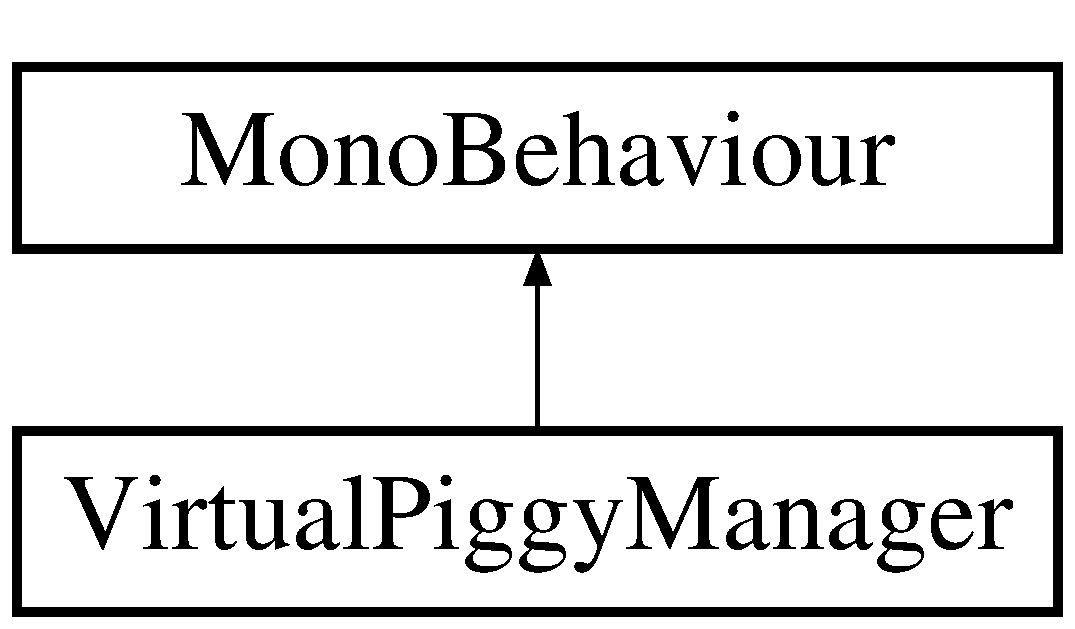
\includegraphics[height=2.000000cm]{class_virtual_piggy_manager}
\end{center}
\end{figure}
\subsection*{Public Member Functions}
\begin{DoxyCompactItemize}
\item 
\hypertarget{class_virtual_piggy_manager_a192474312edf249e11c66badad6da0a3}{void {\bfseries Transaction\-Request} (string product\-Name, float price, int quantity, string product\-Description)}\label{class_virtual_piggy_manager_a192474312edf249e11c66badad6da0a3}

\item 
\hypertarget{class_virtual_piggy_manager_aa2792d32936ebdc9a002f8dfad7b58b2}{void {\bfseries Login\-Request} (string user\-Type, string username, string password)}\label{class_virtual_piggy_manager_aa2792d32936ebdc9a002f8dfad7b58b2}

\end{DoxyCompactItemize}
\subsection*{Properties}
\begin{DoxyCompactItemize}
\item 
\hypertarget{class_virtual_piggy_manager_a18ed56952c5388270eba62e6357bd7b0}{static \hyperlink{class_virtual_piggy_manager}{Virtual\-Piggy\-Manager} {\bfseries Instance}\hspace{0.3cm}{\ttfamily  \mbox{[}get\mbox{]}}}\label{class_virtual_piggy_manager_a18ed56952c5388270eba62e6357bd7b0}

\end{DoxyCompactItemize}


The documentation for this class was generated from the following file\-:\begin{DoxyCompactItemize}
\item 
/\-Users/\-C\-P\-X-\/\-Hackintosh01/\-Virtual Piggy Plugin/\-Assets/\-Plugins/\-Virtual\-Piggy/Virtual\-Piggy\-Manager.\-cs\end{DoxyCompactItemize}

\hypertarget{class_virtual_piggy_settings}{\section{Virtual\-Piggy\-Settings Class Reference}
\label{class_virtual_piggy_settings}\index{Virtual\-Piggy\-Settings@{Virtual\-Piggy\-Settings}}
}


Virtual Piggy Plugin Settings. These are set using the Project Settings window, accessed from Menu Virtual Piggy$>$Project Settings  


\subsection*{Public Types}
\begin{DoxyCompactItemize}
\item 
enum {\bfseries V\-P\-\_\-\-E\-N\-V\-I\-R\-O\-N\-M\-E\-N\-T} \{ {\bfseries D\-E\-V\-E\-L\-O\-P\-M\-E\-N\-T}, 
{\bfseries L\-I\-V\-E}
 \}
\end{DoxyCompactItemize}
\subsection*{Static Public Member Functions}
\begin{DoxyCompactItemize}
\item 
\hypertarget{class_virtual_piggy_settings_a05e4d1aa8d82b9e6f2aba9bff0ab201f}{static void {\bfseries Save\-Settings\-To\-Disk} ()}\label{class_virtual_piggy_settings_a05e4d1aa8d82b9e6f2aba9bff0ab201f}

\item 
\hypertarget{class_virtual_piggy_settings_ab019ab2036fb553ee8db1dfe2d68ac85}{static void {\bfseries Load\-Settings\-From\-Disk} ()}\label{class_virtual_piggy_settings_ab019ab2036fb553ee8db1dfe2d68ac85}

\end{DoxyCompactItemize}
\subsection*{Static Public Attributes}
\begin{DoxyCompactItemize}
\item 
static string \hyperlink{class_virtual_piggy_settings_af24b0af7a500e1e344784a0d209b3fbd}{merchant\-I\-D} = \char`\"{}\char`\"{}
\begin{DoxyCompactList}\small\item\em Virtual Piggy Merchant I\-D. \end{DoxyCompactList}\item 
static string \hyperlink{class_virtual_piggy_settings_a20fd188e30df7a325b9b089af0de683d}{api\-Key} = \char`\"{}\char`\"{}
\begin{DoxyCompactList}\small\item\em Merchant A\-P\-I Key \end{DoxyCompactList}\item 
static V\-P\-\_\-\-E\-N\-V\-I\-R\-O\-N\-M\-E\-N\-T \hyperlink{class_virtual_piggy_settings_aa1795be8074c0d0ef5abfd13bfbf3007}{environment} = V\-P\-\_\-\-E\-N\-V\-I\-R\-O\-N\-M\-E\-N\-T.\-D\-E\-V\-E\-L\-O\-P\-M\-E\-N\-T
\begin{DoxyCompactList}\small\item\em Application environment, if development, will only do test calls to Virtual Piggy back end \end{DoxyCompactList}\end{DoxyCompactItemize}


\subsection{Detailed Description}
Virtual Piggy Plugin Settings. These are set using the Project Settings window, accessed from Menu Virtual Piggy$>$Project Settings 



\subsection{Member Data Documentation}
\hypertarget{class_virtual_piggy_settings_a20fd188e30df7a325b9b089af0de683d}{\index{Virtual\-Piggy\-Settings@{Virtual\-Piggy\-Settings}!api\-Key@{api\-Key}}
\index{api\-Key@{api\-Key}!VirtualPiggySettings@{Virtual\-Piggy\-Settings}}
\subsubsection[{api\-Key}]{\setlength{\rightskip}{0pt plus 5cm}string Virtual\-Piggy\-Settings.\-api\-Key = \char`\"{}\char`\"{}\hspace{0.3cm}{\ttfamily [static]}}}\label{class_virtual_piggy_settings_a20fd188e30df7a325b9b089af0de683d}


Merchant A\-P\-I Key 

\hypertarget{class_virtual_piggy_settings_aa1795be8074c0d0ef5abfd13bfbf3007}{\index{Virtual\-Piggy\-Settings@{Virtual\-Piggy\-Settings}!environment@{environment}}
\index{environment@{environment}!VirtualPiggySettings@{Virtual\-Piggy\-Settings}}
\subsubsection[{environment}]{\setlength{\rightskip}{0pt plus 5cm}V\-P\-\_\-\-E\-N\-V\-I\-R\-O\-N\-M\-E\-N\-T Virtual\-Piggy\-Settings.\-environment = V\-P\-\_\-\-E\-N\-V\-I\-R\-O\-N\-M\-E\-N\-T.\-D\-E\-V\-E\-L\-O\-P\-M\-E\-N\-T\hspace{0.3cm}{\ttfamily [static]}}}\label{class_virtual_piggy_settings_aa1795be8074c0d0ef5abfd13bfbf3007}


Application environment, if development, will only do test calls to Virtual Piggy back end 

\hypertarget{class_virtual_piggy_settings_af24b0af7a500e1e344784a0d209b3fbd}{\index{Virtual\-Piggy\-Settings@{Virtual\-Piggy\-Settings}!merchant\-I\-D@{merchant\-I\-D}}
\index{merchant\-I\-D@{merchant\-I\-D}!VirtualPiggySettings@{Virtual\-Piggy\-Settings}}
\subsubsection[{merchant\-I\-D}]{\setlength{\rightskip}{0pt plus 5cm}string Virtual\-Piggy\-Settings.\-merchant\-I\-D = \char`\"{}\char`\"{}\hspace{0.3cm}{\ttfamily [static]}}}\label{class_virtual_piggy_settings_af24b0af7a500e1e344784a0d209b3fbd}


Virtual Piggy Merchant I\-D. 



The documentation for this class was generated from the following file\-:\begin{DoxyCompactItemize}
\item 
/\-Users/\-C\-P\-X-\/\-Hackintosh01/\-Virtual Piggy Plugin/\-Assets/\-Plugins/\-Virtual\-Piggy/Virtual\-Piggy\-Settings.\-cs\end{DoxyCompactItemize}

\addcontentsline{toc}{part}{Index}
\printindex
\end{document}
